\chapter{Results}
\label{chapter:results}

This last chapter aims to sum up the results coming from the machine-learning modeling of the problem to its modal decomposition.

\section{Domain}

This chapter explains the results from the corner points of the domain made by:

\begin{table}[!h]
\caption{Domain boundary values.}
\label{tab:value}
\begin{center}
    \begin{tabular}{||c l l||} 
        \hline
        \rule{0pt}{10pt} DOF & Min & Max \\ [0.5ex] 
        \hline\hline
        \rule{0pt}{10pt} $\alpha_1$ & $-50.0^{\circ}$ & $-20.0^{\circ}$  \\ 
        \hline
        \rule{0pt}{10pt} $\alpha_2$ & $+65.0^{\circ}$ & $+72.5^{\circ}$ \\
        \hline
        \rule{0pt}{10pt} $M_2$ & $0.4$ & $0.7$ \\
        \hline 
        \rule{0pt}{10pt} $Re$ & $6 \cdot 10^5$ & $6 \cdot 10^5$ \\
        \hline 
        \rule{0pt}{13pt} $\frac{M_{LE}}{M_{TE}}\frac{M_2}{M_1}$ & $1.2$ & $1.8$ \\[4pt]
        \hline 
        \rule{0pt}{13pt} $\frac{M_{PRESS}}{M_{TE}}\frac{M_2}{M_{1, ax}}$ & $0.8$ & $1.0$ \\[4pt] 
        \hline 
        \rule{0pt}{13pt} $\frac{M_{PEAK}}{M_{TE}}$ & $1.2$ & $1.4$ \\[4pt]
        \hline 
        \rule{0pt}{13pt} $\frac{L_{PEAK}}{L_{TOT}}$ & $0.5$ & $0.6$ \\ [4pt] 
        \hline
    \end{tabular}
\end{center}
\end{table}

\section{Optimization Results}

\texttt{TurbOpt} allows to compute the blades that will form the \textbf{boundaries of the domain of study} (in Table~\ref{tab:value}).
The optimization is \textbf{very sensitive to the initial blade} conditions, $\boldsymbol{x}_0$, and reaches \textbf{different blade configurations} with respect to the \textbf{cost function} used in the optimization.

\subsection{Cost Function}

For this optimization, \texttt{TurbOpt} uses the following:

\begin{align}
    RMSE            & = \sqrt{\frac{1}{N_{points}} \cdot \sum_{i = 1}^{N_{points}} \Bigg( \frac{M_{real}}{M_{TE, real}} \Bigg|_{i} - \frac{M_{target}}{M_{TE, target}} \Bigg|_{i} \Bigg)^2} 
    \label{eqn:RMSE} \\ 
    \Delta \alpha_2 & = | \alpha_{2, real} - \alpha_{2, target} | 
    \label{eqn:angleError} \\
    cost            & = RMSE \cdot \Big[ 1 + 0.1 \cdot \Big( max(0.4, \ \Delta \alpha_2) \cdot 2.0 \Big)^{1.5} \Big]
    \label{eqn:costFunction}
\end{align}

The cost function, Equation~(\ref{eqn:costFunction}), is a blend of several flow properties such as the \textbf{root mean square error} over the load along the blade, Equation~(\ref{eqn:RMSE}) , and the \textbf{exit angle error}, Equation~(\ref{eqn:angleError}). 

\subsection{Main Optimized Blades}

The following is a collection of the main optimized blades with respective \textit{consideration} over the optimization and the \textit{validity} of the optimization.

\subsubsection{Overshot on the Peak Mach Fraction}

One of the possible problems that can be encountered in the optimization is that the optimizer cannot generate a blade that follows \textit{perfectly} the aerodynamic style due to \textbf{flow physics}.

\begin{figure}[!ht]
    \centering
    \includegraphics[scale=0.34, page={1}]{figures/optimized/VKIcase005.pdf}
    \includegraphics[scale=0.34, page={2}]{figures/optimized/VKIcase005.pdf}
    \caption{Overshot on the peak Mach fraction even though the optimizer has reached convergence.}
    \label{fig:opt0}
\end{figure}

\subsubsection{$\Delta \alpha_2$ vs Aerodynamic Style}

Another possible problem can be related to the \textbf{unfeasibility} of the \textbf{aerodynamic style} with respect to the \textbf{exit angle error}, $\Delta \alpha_2$, as shown in Figure~\ref{fig:opt1}.

\begin{figure}[!ht]
    \centering
    \includegraphics[scale=0.34, page={1}]{figures/optimized/VKIcase077.pdf}
    \includegraphics[scale=0.34, page={2}]{figures/optimized/VKIcase077.pdf}
    \caption{High error on the exit angle, $\alpha_2$, even though the load follows perfectly the target aerodynamic style.}
    \label{fig:opt1}
\end{figure}

\newpage

\subsubsection{Desired Blade Optimization}

Figure~\ref{fig:opt2} shows a \textit{perfectly} converged blade, \textbf{both} on aerodynamic style and exit angle. This is a clear example of a \textbf{feasible blade design}. The design shown in Figure~\ref{fig:opt0} and Figure~\ref{fig:opt1} are a clear example of the optimization limit due to \textbf{flow physics}.

\begin{figure}[!ht]
    \centering
    \includegraphics[scale=0.34, page={1}]{figures/optimized/VKIcase087.pdf}
    \includegraphics[scale=0.34, page={3}]{figures/optimized/VKIcase087.pdf}
    \caption{Fully converged blade.}
    \label{fig:opt2}
\end{figure}

\subsubsection{\texttt{MISES} Output Validity}

Figure~\ref{fig:opt0}, Figure~\ref{fig:opt1} and Figure~\ref{fig:opt2} already show \texttt{MISES}, \cite{drela2008user}, convergence history\footnote{On the top rigth of the figures.}. 
The following plots are intended to show the \textit{validity} of the simulation plotting the \textbf{blade channel grid} and the \textbf{flow contour plot} for the blade show in Figure~\ref{fig:opt2}:

\begin{figure}[!ht]
    \centering
    \hspace*{-1.5cm}
    \begin{minipage}{0.5\textwidth}
        \includegraphics[scale=0.5, page={5}]{figures/optimized/VKIcase087.pdf}
    \end{minipage}
    \begin{minipage}{0.5\textwidth}
        \includegraphics[scale=0.35, page={6}]{figures/optimized/VKIcase087.pdf}
    \end{minipage}
    \caption{Blade setup.}
\end{figure}
\vspace*{-0.5cm}
\begin{figure}[!ht]
    \centering
    \hspace{2.5cm}
    \includegraphics[scale=0.4, page={7}]{figures/optimized/VKIcase087.pdf}
    \caption{Blade grid.}
    \label{fig:opt3}
\end{figure}

\begin{figure}[!ht]
    % \centering
    \hspace*{-2.0cm}
    \begin{minipage}{0.5\textwidth}
        \includegraphics[scale=0.34, page={13}]{figures/optimized/VKIcase087.pdf}
        \includegraphics[scale=0.34, page={14}]{figures/optimized/VKIcase087.pdf}
        \includegraphics[scale=0.34, page={15}]{figures/optimized/VKIcase087.pdf}
        \caption{Flow contour plot.}
        \label{fig:opt4}
    \end{minipage}
    \hfill
    \begin{minipage}{0.5\textwidth}
        \includegraphics[scale=0.34, page={16}]{figures/optimized/VKIcase087.pdf}
        \includegraphics[scale=0.34, page={17}]{figures/optimized/VKIcase087.pdf}
        \includegraphics[scale=0.34, page={18}]{figures/optimized/VKIcase087.pdf}
        \caption{Flow contour plot.}
        \label{fig:opt5}
    \end{minipage}
\end{figure}

% \begin{figure}[!ht]
    % \centering
    % \includegraphics[scale=0.34, page={16}]{figures/optimized/VKIcase087.pdf}
    % \includegraphics[scale=0.34, page={17}]{figures/optimized/VKIcase087.pdf}
    % \includegraphics[scale=0.34, page={18}]{figures/optimized/VKIcase087.pdf}
    % \caption{Flow contour plot.}
    % \label{fig:opt5}
% \end{figure}

\clearpage

\section{Linear Interpolation of the Domain}
\label{sec:linSec}

A \textit{first attempt} on the \textbf{interpolation of the generated data} has been made over the corner points of the domain. The interpolation is based on a \textbf{linear interpolation}\footnote{The interpolation has been generated using the \href{https://docs.scipy.org/doc/scipy/reference/interpolate.html}{scipy.interpolate} module.}. It takes a linear variation of the blade geometry over the \textbf{aerodynamic style} and the \textbf{aerodynamic duty}. The main blade features are plotted hereafter.

\begin{figure}[!ht]
    \centering
    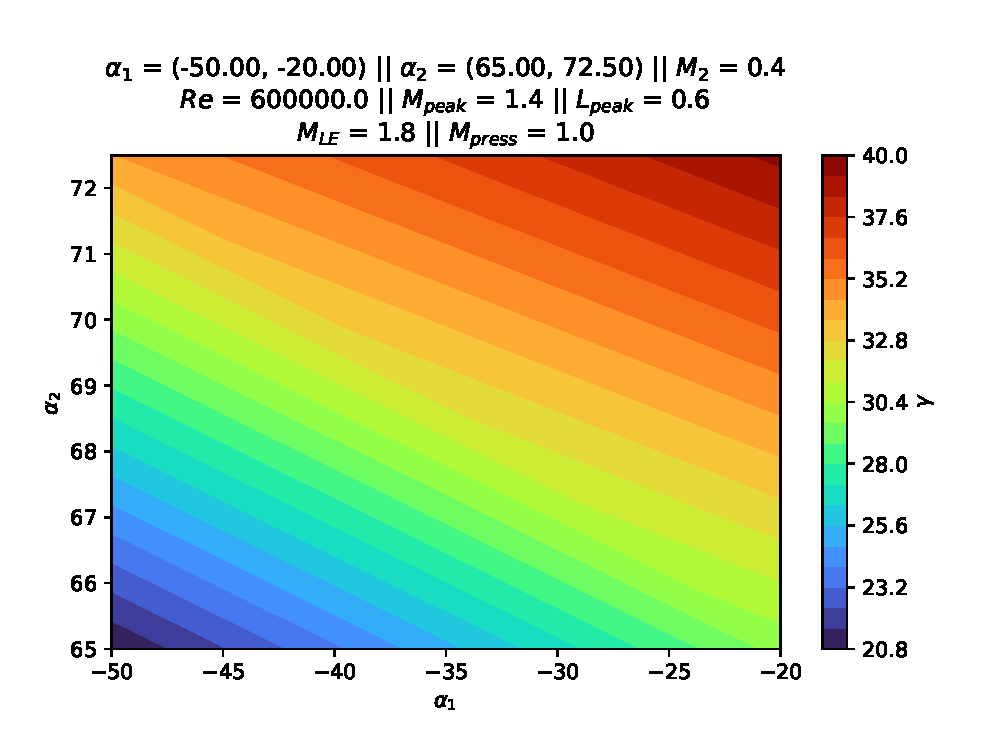
\includegraphics[scale=0.7]{figures/interpolation/alpha1alpha2stagger.eps}
    \caption{$\gamma$ variation over $\alpha_1$ and $\alpha_2$.}
\end{figure}

\begin{figure}[!ht]
    \centering
    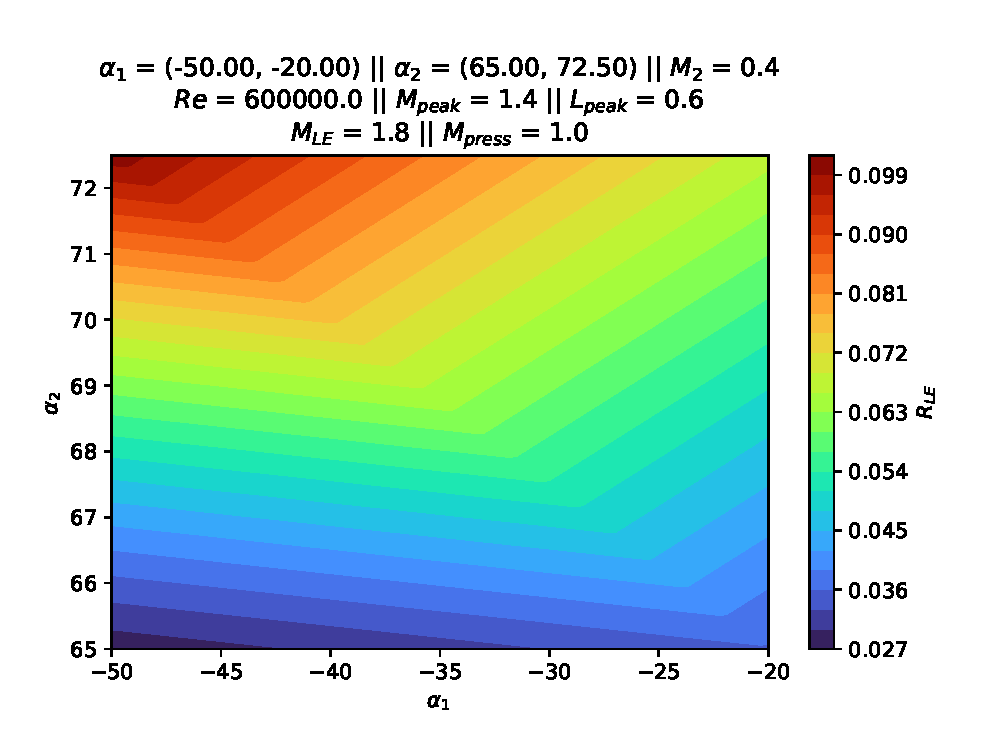
\includegraphics[scale=0.7]{figures/interpolation/alpha1alpha2LEradius.eps}
    \caption{$R_{LE}(A_0)$ variation over $\alpha_1$ and $\alpha_2$.}
\end{figure}

\begin{figure}[!ht]
    \centering
    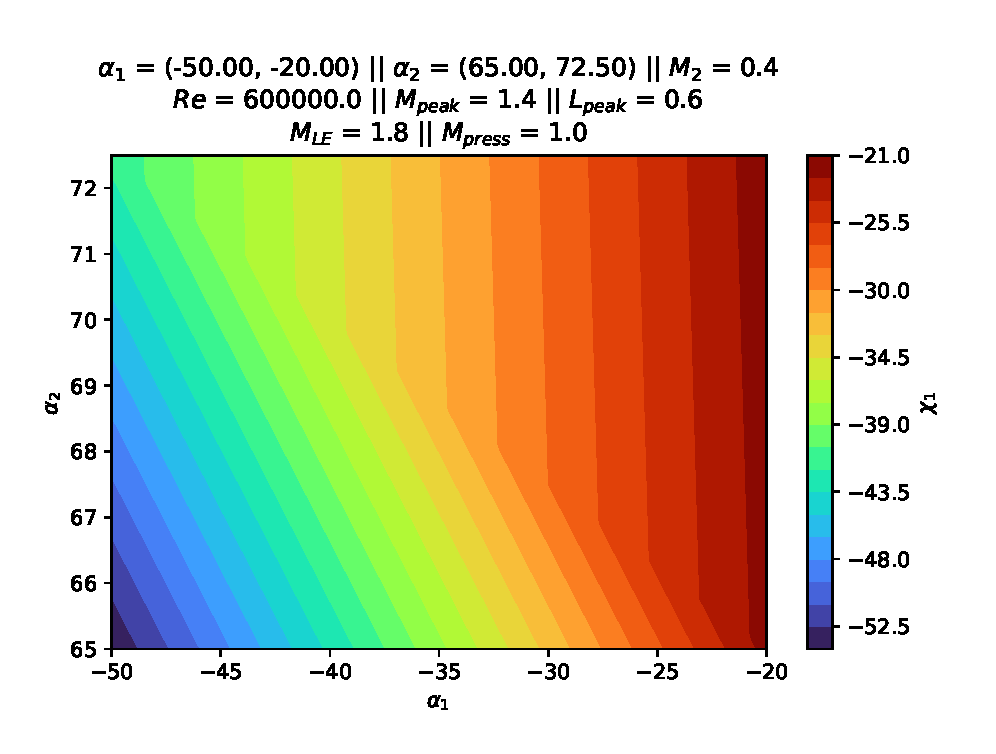
\includegraphics[scale=0.7]{figures/interpolation/alpha1alpha2metalIn.eps}
    \caption{$\chi_1$ variation over $\alpha_1$ and $\alpha_2$.}
\end{figure}

\begin{figure}[!ht]
    \centering
    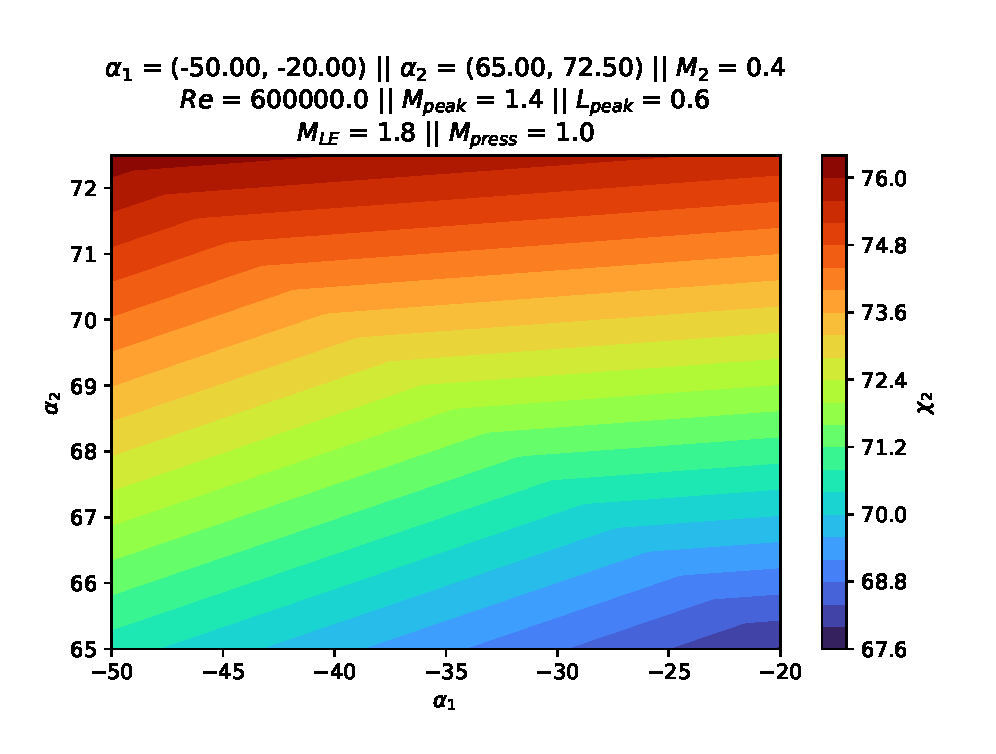
\includegraphics[scale=0.7]{figures/interpolation/alpha1alpha2metalOut.eps}
    \caption{$\chi_2$ variation over $\alpha_1$ and $\alpha_2$.}
\end{figure}

\clearpage

\section{Linear Interpolation of the Error}

As done in Section~\ref{sec:linSec}, a representation of the error, $RMSE$ and $\Delta \alpha_2$, is plotted over the main \textbf{aerodynamic duty} quantities.

\begin{figure}[!ht]
    \centering
    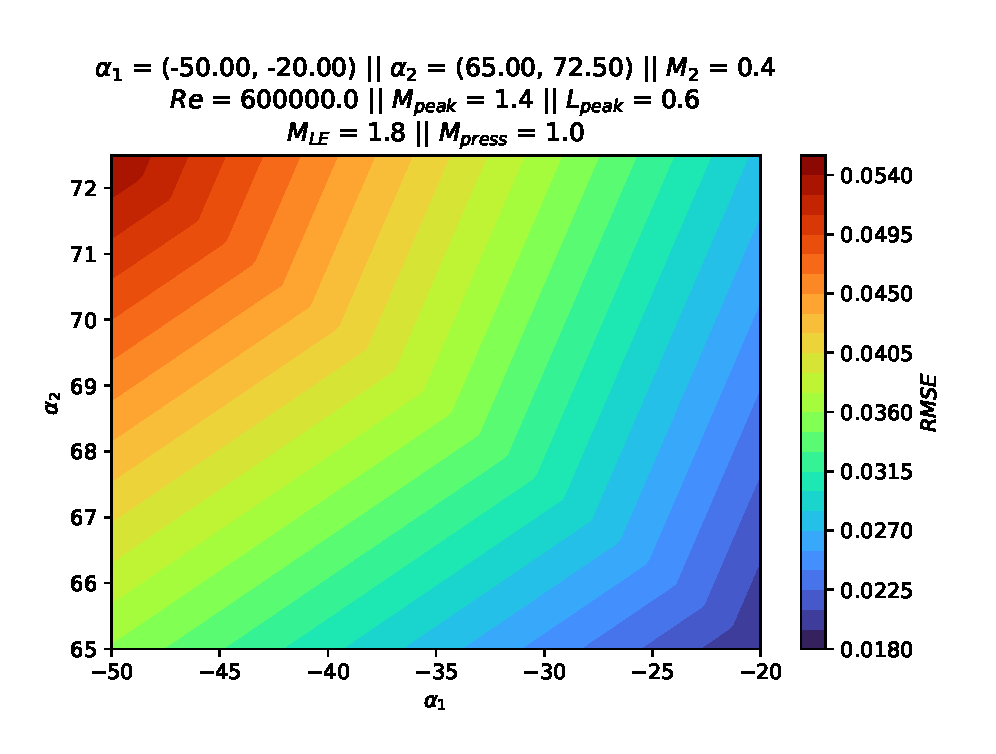
\includegraphics[scale=0.7]{figures/interpolation/alpha1alpha2RMSE.eps}
    \caption{$RMSE$ variation over $\alpha_1$ and $\alpha_2$.}
\end{figure}

\begin{figure}[!ht]
    \centering
    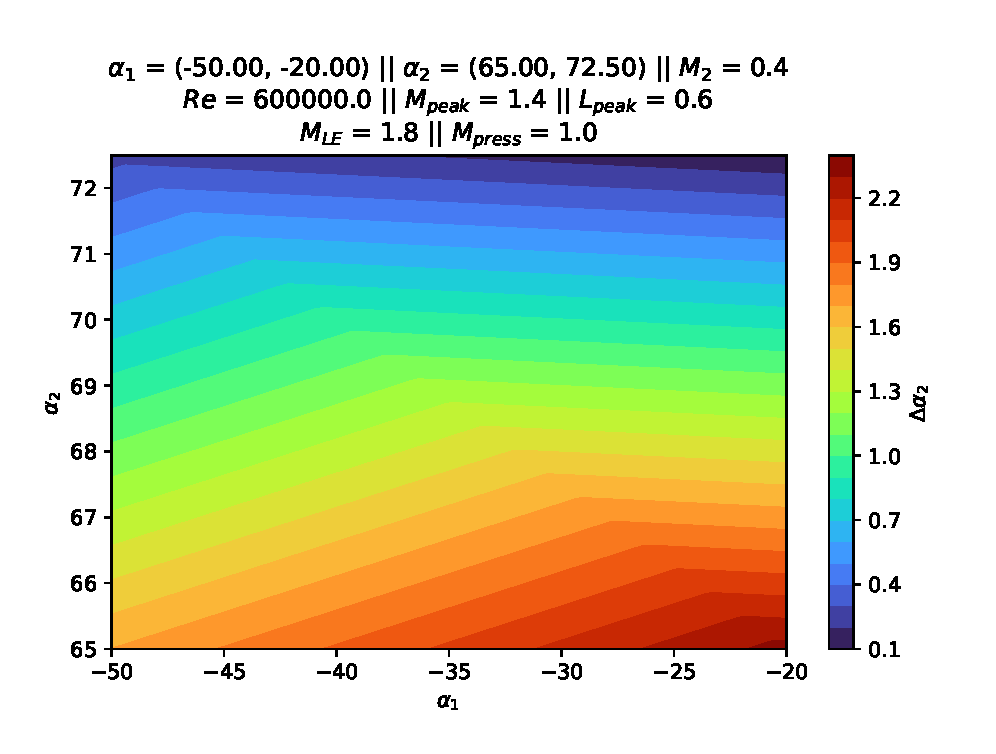
\includegraphics[scale=0.7]{figures/interpolation/alpha1alpha2AlphaError.eps}
    \caption{$\Delta \alpha_2$ variation over $\alpha_1$ and $\alpha_2$.}
\end{figure}